\chapter{Basic usage}
\label{chap:Basic usage}

\section{Conventions}
\label{sec:Conventions}

All classes and functions that are accessible to users are within the name
space \verb|vsmc|. Class names are in \verb|CamelCase| and function names and
class members are in \verb|small_cases|. We will use ``function'' for referring
to name space scope functions and ``method'' for class member functions. For
brevity, we will omit the ``\verb|vsmc::|'' qualifier in the remaining of this
document except in showing complete examples.

\section{Getting and installing the library}
\label{sec:Getting and installing the library}

The library is hosted at
GitHub\footnote{\url{https://github.com/zhouyan/vSMC}}. This is a header only
\cpp template library. To install the library just move the contents of the
\verb|include| directory into a proper place, e.g., \verb|/usr/local/include|
on Unix-alike systems. This library requires working \cppoo and \blas
implementations. Intel Threading Building
Blocks\footnote{\url{https://www.threadingbuildingblocks.org}} (\tbb), Intel
Math Kernel Library\footnote{\url{https://software.intel.com/en-us/intel-mkl}}
(\mkl) and \hdf\footnote{\url{http://www.hdfgroup.org}} are optional
third-party libraries. One need to define the configuration macros
\verb|VSMC_HAS_TBB|, \verb|VSMC_HAS_MKL| and \verb|VSMC_HAS_HDF5|,
respectively, to nonzero values before including any \vsmc headers to make
their existence known to the library.

\section{Concepts}
\label{sec:Concepts}

The library is structured around a few core concepts. A sampler is responsible
for running an algorithm. It contains a particle system and operations on it. A
particle system is formed by the states $\{X^{(i)}\}_{i=1}^N$ and weights
$\{W^{(i)}\}_{i=1}^N$. This system will also be responsible for resampling. All
user defined operations are to be applied to the whole system. These are
``initialization'' and ``moves'' which are applied before resampling, and
``\mcmc'' moves which are applied after resampling. These operations do not
have to be \mcmc kernels. They can be used for any purpose that suits the
particular algorithm. Most statistical inferences requires calculation of
$\sum_{i=1}^NW^{(i)}\varphi(X^{(i)})$ for some function $\varphi$. This can be
carried out along each sampler iteration by a monitor. Table~\ref{tab:concepts}
lists these concepts and the corresponding types in the library. Each of them
are introduced in detail in the following sections.

\begin{table}
  \begin{tabularx}{\textwidth}{lL}
    \toprule
    Concept & Type \\
    \midrule
    State, $\{X^{(i)}\}_{i=1}^N$            & \verb|T|, user defined   \\
    Weight, $\{W^{(i)}\}_{i=1}^N$           & \verb|Weight|            \\
    Particle, $\{W^{(i)},X^{(i)}\}_{i=1}^N$ & \verb|Particle<T>|       \\
    Single particle, $\{W^{(i)},X^{(i)}\}$  & \verb|SingleParticle<T>| \\
    Sampler        & \verb|Sampler<T>|                                 \\
    Initialization & \verb|Sampler<T>::init_type|, user defined        \\
    Move           & \verb|Sampler<T>::move_type|, user defined        \\
    \mcmc          & \verb|Sampler<T>::mcmc_type|, user defined        \\
    Monitor        & \verb|Monitor<T>|                                 \\
    \bottomrule
  \end{tabularx}
  \caption{Core concepts of the library}
  \label{tab:concepts}
\end{table}

\subsection{State}
\label{sub:State}

The library gives users the maximum flexibility of how the states
$\{X^{(i)}\}_{i=1}^N$ shall be stored and structured. Any class type with a
constructor that takes a single integer value, the number of particles, as its
argument, and a method named \verb|copy| is acceptable. For example,
\begin{Verbatim}
  class T
  {
      public:
      T(std::size_t N);

      template <typename IntType>
      void copy(std::size_t N, IntType *index)
      {
          for (std::size_t i = 0; i != N; ++i) {
              // Let $a_i =$ index[i], set $X^{(i)} = X^{(a_i)}$
          }
      }
  };
\end{Verbatim}
How the state values are actually stored and accessed are entirely up to the
user. The method \verb|copy| is necessary since the library assumes no
knowledge of the internal structure of the state. And thus it cannot perform
the last step of a resampling algorithm, which makes copies of particles with
larger weights and eliminate those with smaller weights.

\subsubsection{The \texttt{StateMatrix} class template}

For most applications, the values can be stored within an $N$ by $d$ matrix,
where $d$ is the dimension of the state. The library provides a convenient
class template for this situation,
\begin{Verbatim}
  template <MatrixLayout Layout, std::size_t Dim, typename T>
  class StateMatrix;
\end{Verbatim}
where \verb|Layout| is either \verb|RowMajor| or \verb|ColMajor|, which
specifies the matrix storage layout; \verb|Dim| is a non-negative integer
value. If \verb|Dim| is zero, then the dimension may be changed at runtime. If
it is positive, then the dimension is fixed and cannot be changed at runtime.
The last template parameter \verb|T| is the \cpp type of state space. The
following constructs an object of this class,
\begin{Verbatim}
  StateMatrix<ColMajor, Dynamic, double> s(N);
\end{Verbatim}
where \verb|Dynamic| is just an enumerator with value zero. We can specify the
dimension at runtime through the method \verb|s.resize_dim(d)|. Note that, if
the template parameter \verb|Dim| is positive, then this call results in a
compile-time error.

To access $X_{ij}$, the value of the state of the $i$\ith particle at the
$j$\ith coordinate, one can use the method \verb|s.state(i,j)|. The method
\verb|s.data()| returns a pointer to the beginning of the matrix. If
\verb|Layout| is \verb|RowMajor|, then the method \verb|s.row_data(i)| returns
a pointer to the beginning of the $i$\ith row. If \verb|Layout| is
\verb|ColMajor|, then the method \verb|s.col_data(j)| returns a pointer to the
beginning of the $j$\ith column. These methods help interfacing with numerical
libraries, such as \blas.

Apart from \verb|resize_dim|, the matrix can also be resized by the sample size
or both. \verb|s.resize(N, dim)| is the most general form. Let $n$ be the
minimum of the original and new sample sizes, and $d$ be the minimum of the
original and new dimensions. The $n$ by $d$ matrix at the upper left corner of
the original matrix is preserved. If the matrix is enlarged in either
direction, new values will be inserted and default initialized. Note that, if
the template parameter \verb|Dim| is positive, then this call results in a
compile-time error. The method call \verb|s.resize(N)| is equivalent to
\verb|s.resize(N, s.dim())| except that it never generate a compile-time error.
For more sophisticated resizing, use the \verb|copy| method, which will create
a new set of states according to the index vector.

\paragraph{Choice between matrix storage layout}

If one needs to access the matrix frequently row by row or column by column,
then the choice of the first template parameter \verb|Layout| is obvious. The
\verb|copy| method, which is used by resampling algorithms, is more efficient
with \verb|RowMajor|. The difference is more significant with large sample
size, high dimension or both. The performance of resizing, either explicitly or
implicitly through \verb|copy|, depends on both the matrix storage layout, the
new sample size and dimension. If the dimension does not change, it is more
efficient to use \verb|RowMajor|. If the sample size does not change, it is
more efficient to use the \verb|ColMajor|. If both of them are changed, then
the performance depends on the original and new sizes.

\subsection{Weight}
\label{sub:Weight}

The vector of weights $\{W^{(i)}\}_{i=1}^N$ is abstracted in the library by the
\verb|Weight| class. The following constructs an object of this class,
\begin{Verbatim}
  Weight w(N);
\end{Verbatim}
There are a few methods for accessing the weights,
\begin{Verbatim}
  w.ess();          // Get {\normalfont\textsc{ess}}
  w.set_equal();    // Set $W^{(i)} = 1/N$
\end{Verbatim}
The weights can be manipulated, given a vector of length $N$, say $v$,
\begin{Verbatim}
  w.set(v);         // Set $W^{(i)} \propto v^{(i)}$
  w.mul(v);         // Set $W^{(i)} \propto W^{(i)} v^{(i)}$
  w.set_log(v);     // Set $\log W^{(i)} = v^{(i)} + \text{const.}$
  w.add_log(v);     // Set $\log W^{(i)} = \log W^{(i)} + v^{(i)} + \text{const.}$
\end{Verbatim}
The method \verb|w.data()| returns a pointer to the normalized weights. It is
important to note that the weights are always normalized and all mutable
methods only allow access to $\{W^{(i)}\}_{i=1}^N$ as a whole.

\subsection{Particle}
\label{sub:Particle}

A particle system is composed of both the state values, which is of user
defined type, say \verb|T|, and the weights. The following constructs an object
of class \verb|Particle<T>|,
\begin{Verbatim}
  Particle<T> particle(N);
\end{Verbatim}
The method \verb|particle.value()| returns the type \verb|T| object. The object
containing the weights is returned by \verb|particle.weight()|. Its type is
\verb|Particle<T>::weight_type|, whose definition depends on the type \verb|T|.
See section~\ref{sec:Customizing member types} for more details. If the user
does not do something special as shown in that section, then the default type
is \verb|Weight|. They are constructed with the same integer value $N$ when the
above constructor is invoked.

For Monte Carlo algorithm, random number generators (\rng) will be used
frequently. The user is free to use whatever \rng mechanism as they see fit.
However, one common issue encountered in practice is how to maintain
independence of the \rng streams between function calls. For example, consider
below a function that manipulates some state values,
\begin{Verbatim}
  void function(double &x)
  {
      std::mt19937 rng;
      std::normal_distribution<double> rnorm(0, 1);
      x = rnorm(rng);
  }
\end{Verbatim}
Every call of this function will give \verb|x| exactly the same value. This is
hardly what the user intended. One might consider an global \rng or one as
class member data. For example,
\begin{Verbatim}
  std::mt19937 rng;

  void function(double &x)
  {
      std::normal_distribution<double> rnorm(0, 1);
      x = rnorm(rng);
  }
\end{Verbatim}
This will work fine as long as the function is never called by two threads at
the same time. However, \smc algorithms are natural candidates to
parallelization. Therefore, the user will need to either lock the \rng, which
degenerates the performance, or construct different \rng{}s for different
threads. The later, though ensures thread-safety, has other issues. For
example, consider
\begin{Verbatim}
  std::mt19937 rng1(s1); // For thread $i_1$ with seed $s_1$
  std::mt19937 rng2(s2); // For thread $i_2$ with seed $s_2$
\end{Verbatim}
where the seeds $s_1 \ne s_2$. It is difficult to ensure that the two streams
generated by the two \rng{}s are independent. Common practice for parallel \rng
is to use sub-streams or leap-frog algorithms. Without going into any further
details, it is sufficient to say that this is perhaps not a problem that most
users bother to solve.

The library provides a simple solution to this issue. The method
\verb|particle.rng(i)| returns a reference to an \rng that conforms to the
\cppoo uniform \rng concept. It can be called from different threads at the
same time, for example,
\begin{Verbatim}
  auto &rng1 = particle.rng(i1); // Called from thread $i_1$
  auto &rng2 = particle.rng(i2); // Called from thread $i_2$
\end{Verbatim}
If $i_1 \ne i_2$, then the subsequent use of the two \rng{}s are guaranteed to
be thread-safe. In addition, they will produce independent streams. If \tbb is
available to the library, then it is also thread-safe even if $i_1 = i_2$. One
can write functions that process each particle, for example,
\begin{Verbatim}
  void function(std::size_t i)
  {
      auto &rng = particle.rng(i);
      // Process the particle i using rng
  }
\end{Verbatim}
And if later this function is called from a parallelized environment, it is
still thread-safe and produce desired statistical results. The details of the
\rng system are documented later in chapter~\ref{chap:Random number
  generating}.

\subsubsection{Resize the particle system}

The particle system can be resized. However, the library does not provide a
simple \verb|resize| method that works the same way as \verb|std::vector|, etc.
When a particle system is resized, it is often done through some deterministic
or stochastic algorithms. At least some particles will be preserved and
possibly replicated. The \verb|Particle<T>| class has a few methods for
resizing using different user input to determine the particles to be preserved.
All these methods use \verb|T::copy| to resize the state vector. Therefore, if
any of them need to be used, the method call \verb|copy(N, index)| need to be
able to handle the situation where its first argument has a value other than
its original size. After the resizing, the weights are set to be equal.

\paragraph{Resize by selecting according to a user supplied index vector}

\begin{Verbatim}
  template <typename InputIter>
  void resize_by_index(size_type N, InputIter index);
\end{Verbatim}
The input iterator \verb|index| shall point to a length $N$ vector. Each
element is the parent index of the corresponding new particle. The new system
is formed by $\bar{X}^{(i)} = X^{(a_i)}$ where $a_i$ is the $i$\ith element of
the index vector.

\paragraph{Resize by selecting according to a user supplied mask vector}

\begin{Verbatim}
  template <typename InputIter>
  void resize_by_mask(size_type N, InputIter mask);
\end{Verbatim}
The input iterator \verb|mask| shall point to a length $n$ vector, where $n$ is
the original sample size. For each element, when converted to \verb|bool|, if
it is \verb|true|, then the corresponding particle is preserved. Otherwise it
is discarded. If there are more than $N$ particles to be preserved, then only
the first $N$ particles are copied into the new system. If there are less than
$N$ particles to be preserved, then the vector of these particles are copied
repeatedly until there are enough particles to fill the new system.

\paragraph{Resize by resampling}

\begin{Verbatim}
  template <typename ResampleType>
  void resize_by_resample(size_type N, ResampleType &&op);
\end{Verbatim}
The details of the resampling operation function object is discussed in
chapter~\ref{chap:Resampling}. For now, it is sufficient to say that, to use
any of the builtin schemes, one can call the method like the following,
\begin{Verbatim}
  particle.resize_by_resample(N, ResampleMultinomial());
\end{Verbatim}
This method produce a new particle system by using the specified resampling
algorithm. Note that, this is different from resampling a particle system in
that, all operations are local. That is, if the particle is in a distributed
system, only local weights are used, and re-normalized.

\paragraph{Resize by uniformly selecting from all particles}

\begin{Verbatim}
  void resize_by_uniform(size_type N);
\end{Verbatim}
This is equivalent to,
\begin{Verbatim}
  particle.weight().set_equal();
  particle.resize_by_resample(N, ResampleMultinomial());
\end{Verbatim}

\paragraph{Resize by selecting a range of particles}

\begin{Verbatim}
  void resize_by_range(size_type N, size_type first, size_type last);
\end{Verbatim}
This is the most destructive resizing method. Let $n = \text{last} -
\text{first}$. If $n < N$, the particles in the range $[\text{first},
\text{last})$ are copied repeatedly until there are enough particles to fill
the new system. Otherwise only the first $N$ particles are copied. If
\verb|last| is omitted, then it is set to \verb|size()|. If \verb|first| is
also omitted, then it is set to zero. Use this method only when the statistical
properties of the new system is irrelevant. If one want to avoid the copying
altogether, it might be more efficient to simply create a new system with
the desired size. This method is a no-op if $N$ is the same as the original
size.

\subsection{Single particle}
\label{sub:Single particle}

It is often easier to define a function $f(X^{(i)})$ than
$f(X^{(1)},\dots,X^{(N)})$. However, \verb|Particle<T>| only provides access to
$\{X^{(i)}\}_{i=1}^N$ as a whole through \verb|particle.value()|. To allow
direct access to $X^{(i)}$, the library uses a class \verb|SingeParticle<T>|.
An object of this class is constructed from the index $i$ of the particle, and
a pointer to the particle system it belongs to,
\begin{Verbatim}
  SingleParticle<T> sp(i, &particle);
\end{Verbatim}
or more conveniently,
\begin{Verbatim}
  auto sp = particle.sp(i);
\end{Verbatim}
In its most basic form, it has the following methods,
\begin{Verbatim}
  sp.id();       // Get the value i that sp was constructed with
  sp.particle(); // Get a reference to the Particle<T> object sp belongs to
  sp.rng();      // => sp.particle().rng(sp.id());
\end{Verbatim}
If \verb|T| is a derived class of \verb|StateMatrix|, then it has two
additional methods,
\begin{Verbatim}
  sp.dim();    // => sp.particle().value().dim();
  sp.state(j); // => sp.particle().value().state(sp.id(), j);
\end{Verbatim}
It is clear now that the interface of \verb|SingleParticle<T>| depends on the
type \verb|T|. Later in section~\ref{sec:Extending SP} we will show how to
insert additional methods into this class.

A \verb|SingleParticle<T>| object is similar to an iterator. In fact, it
supports almost all of the operations of a random access iterator with two
exceptions. First dereferencing a \verb|SingleParticle<T>| object returns
itself. The support of \verb|operator*| allows the range-based for loop to be
applied on a \verb|Particle<T>| object, for example,
\begin{Verbatim}
  for (auto sp : particle) {
      // operations on sp
  }
\end{Verbatim}
is equivalent to
\begin{Verbatim}
  for (std::size_t i = 0; i != particle.size(); ++i) {
      auto sp = particle.sp(i);
      // operations on sp
  }
\end{Verbatim}
The above range-based loop does make some sense. However trying to
dereferencing a \verb|SingleParticle<T>| object in other contexts does not make
much sense. Recall that it is an \emph{index}, not a \emph{pointer}. The
library does not require the user defined type \verb|T| to provide access to
individual values, and thus it cannot dereference a \verb|SingleParticle<T>|
object to obtain such a value. Similarly, the expression \verb|sp[n]| returns
\verb|sp + n|, another \verb|SingleParticle<T>| object. For the same reason,
\verb|operator->| is not supported at all.

\subsection{Sampler}
\label{sub:Sampler}

A sampler can be constructed in a few ways,
\begin{Verbatim}
  Sampler<T> sampler(N);
\end{Verbatim}
constructs a sampler that is never resampled, while
\begin{Verbatim}
  Sampler<T> sampler(N, Multinomial);
\end{Verbatim}
constructs a sampler that is resampled every iteration, using the Multinomial
algorithm. Other resampling schemes are also implemented, see
chapter~\ref{chap:Resampling}. Last, one can also construct a sampler that is
only resampled when $\ess < \alpha N$, where $\alpha\in[0, 1]$, by the
following,
\begin{Verbatim}
  Sampler<T> sampler(N, Multinomial, alpha);
\end{Verbatim}
If $\alpha > 1$, then it has the same effect as the first constructor, since
$\ess \le N$. If $\alpha < 0$, then it has the same effect as the second
constructor, since $\ess > 0$.

In summary, if one does not tell the constructor which resampling scheme to
use, then it is assumed one does not want to do resampling. If one specify the
resampling scheme without a threshold for \ess, then it is assumed it need to
be done at every step.

The method \verb|sampler.particle()| returns a reference to the particle
system. It is safe to resize a \verb|Particle<T>| object contained within a
\verb|Sampler<T>| object. The method \verb|sampler.size()| is only a shortcut
to \verb|sampler.particle().size()|.

A sampler can be initialized by user defined function objects that are
convertible to the following type,
\begin{Verbatim}
  using init_type = std::function<std::size_t(Particle<T> &, void *)>;
\end{Verbatim}
For example,
\begin{Verbatim}
  auto init = [](Particle<T> &particle, void *param) {
      // Process initialization parameter param
      // Initialize the particle system particle
  };
\end{Verbatim}
is a \cppoo lambda expression that can be used for this purpose. One can add it
to a sampler by calling \verb|sampler.init(init)|. Upon calling
\verb|sampler.initialize(param)|, the user defined \verb|init| will be called
and the argument \verb|param| will be passed to it.

Similarly, after initialization, at each iteration, the particle system can be
manipulated by user defined function objects that are convertible to the
following types,
\begin{Verbatim}
  using move_type = std::function<std::size_t(std::size_t, Particle<T> &)>;
\end{Verbatim}
Multiple moves can be added to a sampler. The call
\verb|sampler.move(move, append)| adds a \verb|move_type| object to the
sampler, where \verb|append| is a boolean value. If it is \verb|false|, it will
clear any moves that were added before. If it is \verb|true|, then \verb|move|
is appended to the end of an existing sequence of moves. Each move will be
called one by one upon calling \verb|sampler.iterate()|. A similar sequence of
\mcmc moves can also be added to a sampler. The call \verb|sampler.iterate()|
will call user defined moves first, then perform the possible resampling, and
then the sequence of \mcmc moves.

Note that the possible resampling will also be performed after the user defined
initialization function is called by \verb|sampler.initialize(param)|. And
after that, the sequence of \mcmc moves will be called. If it desired not to
perform mutations during initialization, then following can be used,
\begin{Verbatim}
  sampler.init(init).initialize(param);
  sampler.move(move, false).mcmc(mcmc, false).iterate(n);
\end{Verbatim}
The above code also demonstrates that most methods of \verb|Sampler<T>| return
a reference to the sampler itself and thus method calls can be chained. In
addition, method \verb|sampler.iterate(n)| accepts an optional argument that
specifies the number of iterations. It is a shortcut for
\begin{Verbatim}
  for (std::size_t i = 0; i != n; ++i)
      sampler.iterate();
\end{Verbatim}

\subsection{Monitor}
\label{sub:Monitor}

Inferences using a \smc algorithm usually require the calculation of the
quantity $\sum_{i=1}^NW^{(i)}\varphi(X^{(i)})$ at each iteration for some
function $\varphi$. One can define function objects that are convertible to the
following type,
\begin{Verbatim}
  using eval_type =
      std::function<void(std::size_t, std::size_t, Particle<T> &, double *);
\end{Verbatim}
For example,
\begin{Verbatim}
  void eval(std::size_t iter, std::size_t d, Particle<T> &particle, double *r)
  {
      for (std::size_t i = 0; i != particle.size(); ++i, r += dim) {
          auto sp = particle.sp(i);
          r[0] = /* $\varphi_1(X^{(i)})$ */;
          // ...
          r[d - 1] = /* $\varphi_d(X^{(i)})$ */;
      }
  }
\end{Verbatim}
The argument \verb|d| is the dimension of the vector function $\varphi$. The
output is an $N$ by $d$ matrix in row major layout, with each row corresponding
to the value of $\varphi(X^{(i)})$. Then one can add this function to a sampler
by calling,
\begin{Verbatim}
  sampler.monitor("name", d, eval);
\end{Verbatim}
where the first argument is the name for the monitor; the second is the
dimension to be passed to the user defined function; and the third is the
evaluation function. At each iteration, after all the initialization, possible
resampling, moves and \mcmc moves are done, the sampler will calculate
$\sum_{i=1}^NW^{(i)}\varphi(X^{(i)})$. This method has two optional arguments.
The first is a boolean value \verb|record_only|. If it is \verb|true|, it is
assumed that no summation is needed. For example,
\begin{Verbatim}
  void eval(std::size_t iter, std::size_t d, Particle<T> &particle, double *r)
  {
      r[0] = /* $\varphi_1(\{X^{(i)}\}_{i=1}^N)$ */;
      // ...
      r[d - 1] = /* $\varphi_d(\{X^{(i)}\}_{i=1}^N)$ */;
  }
\end{Verbatim}
In this case, the monitor acts merely as a storage facility. The second
optional argument is \verb|stage| which specifies at which point the monitoring
shall happen. It can be \verb|MonitorMove|, which specifies that the monitoring
happens right after the moves and before resampling. It can also be
\verb|MonitorResample|, which specifies that the monitoring happens right after
the resampling and before the \mcmc moves. Last, the default is
\verb|MonitorMCMC|, which specifies that the monitoring happens after
everything.

The output of a sampler, together with the records of any monitors it has can
be output in plain text forms through a \cpp output stream. For example,
\begin{Verbatim}
  std::cout << sampler;
\end{Verbatim}
We will see how this works later with a concrete particle filter example. If
the \hdf library is available, it is also possible to write such output to \hdf
format, for example,
\begin{Verbatim}
  hdf5store(sampler, file_name, data_name);
\end{Verbatim}
Details can be found in section~\ref{sec:Store objects in HDF5 format}. More
sophisticated methods for retrieving monitor records are defined by the
\verb|Monitor<T>| class. An object of this class can be retrieved by
\verb|sampler.monitor("name")|. See the reference manual for details.

\section{A simple particle filter}
\label{sec:A simple particle filter}

\subsection{Model and algorithm}
\label{sub:Model and algorithm}

This is an example used in \textcite{Johansen:2009wd}. Through this example, we
will show how to re-implement a simple particle filter in \vsmc. It shall walk
one through the basic features of the library introduced above.

The state space model, known as the almost constant velocity model in the
tracking literature, provides a simple scenario. The state vector $X_t$
contains the position and velocity of an object moving in a plane. That is,
$X_t = (\xpos^t, \ypos^t, \xvel^t, \yvel^t)^T$. Imperfect observations $Y_t =
(\xobs^t, \yobs^t)^T$ of the positions are possible at each time instance. The
state and observation equations are linear with additive noises,
\begin{align*}
  X_t &= AX_{t-1} + V_t \\
  Y_t &= BX_t + \alpha W_t
\end{align*}
where
\begin{equation*}
  A = \begin{pmatrix}
    1 & 0 & \Delta & 0      \\
    0 & 1 & 0      & \Delta \\
    0 & 0 & 1      & 0      \\
    0 & 0 & 0      & 1
  \end{pmatrix} \qquad
  B = \begin{pmatrix}
    1 & 0 & 0 & 0 \\
    0 & 1 & 0 & 0 \\
  \end{pmatrix} \qquad
  \alpha = 0.1
\end{equation*}
and we assume that the elements of the noise vector $V_t$ are independent
Gaussian with variance $0.02$ and $0.001$ for position and velocity,
respectively. The observation noise, $W_t$ comprises independent, identically
distributed $t$-distributed random variables with degree of freedom $\nu = 10$.
The prior at time $0$ corresponds to an axis-aligned Gaussian with variance $4$
for the position coordinates and $1$ for the velocity coordinates. The particle
filter algorithm is shown in algorithm~\ref{alg:pf}.

\begin{algorithm}[t]
  \begin{algorithmic}
    \hrule\vskip1ex
    \STATE \emph{Initialization}
    \STATE\STATESKIP Set $t\leftarrow0$.
    \STATE\STATESKIP Sample
    $\xpos^{(0,i)},\ypos^{(0,i)}\sim\calN(0,4)$ and
    $\xvel^{(0,i)},\yvel^{(0,i)}\sim\calN(0,1)$.
    \STATE\STATESKIP Weight $W_0^{(i)} \propto \exp{\ell(X_0^{(i)}|Y_0)}$ where
    $\ell$ is the log-likelihood function.

    \STATE \emph{Iteration}
    \STATE\STATESKIP Set $t\leftarrow t + 1$.
    \STATE\STATESKIP Sample
    \begin{align*}
      \xpos^{(t,i)}&\sim\calN(\xpos^{(t-1,i)} + \Delta\xvel^{(t-1,i)}, 0.02) &
      \xvel^{(t,i)}&\sim\calN(\xvel^{(t-1,i)}, 0.001) \\
      \ypos^{(t,i)}&\sim\calN(\ypos^{(t-1,i)} + \Delta\yvel^{(t-1,i)}, 0.02) &
      \yvel^{(t,i)}&\sim\calN(\yvel^{(t-1,i)}, 0.001)
    \end{align*}
    \STATE\STATESKIP Weight $W_t^{(i)} \propto
    W_{t-1}^{(i)}\exp{\ell(X_t^{(i)}|Y_t)}$.

    \STATE \emph{Repeat the \emph{Iteration} step until all data are processed}.
    \vskip1ex\hrule
  \end{algorithmic}
  \caption{Particle filter algorithm for the almost constant velocity model.}
  \label{alg:pf}
\end{algorithm}

\subsection{Implementations}
\label{sub:Implementations}

The complete program is shown in appendix~\appref{app:sub:Sequential
  implementation}. In this section we show the outline of the implementation.

\subsubsection{The main program}

\begin{Verbatim}
    Sampler<PFState> sampler(N, Multinomial, 0.5);
    sampler.init(PFInit()).move(PFMove(), false).monitor("pos", 2, PFEval());

    sampler.initialize(const_cast<char *>("pf.data")).iterate(n - 1);

    std::ofstream output("pf.out");
    output << sampler;
    output.close();
\end{Verbatim}
\verb|Sampler<PFState>| object is constructed first. Then the initialization
\verb|PFInit|, move \verb|PFMove| and a monitor \verb|PFEval| that records
$\xpos^t$ and $\ypos^t$ are added to the sampler. The monitor is named
\verb|"pos"|. Then it is initialized with the name of the data file
\verb|"pf.data"|, and iterated $n - 1$ times, where $n$ is the number of data
points. At last, the output is written into a text file \verb|"pf.out"|. Below
is a short R\footnote{\url{http://r-project.org}} script that can be used to
process the output
\begin{Verbatim}
  pf <- read.table("pf.out", header = TRUE)
  print(pf[1:5,])
\end{Verbatim}
The \verb|print(pf[1:5,])| statement shows the first five lines of the output,
\begin{Verbatim}
    Size Resampled Accept.0      ESS    pos.0   pos.1
  1 1000         1        0   2.9204 -1.21951 3.16397
  2 1000         1        0 313.6830 -1.15602 3.22770
  3 1000         1        0  33.0421 -1.26451 3.04031
  4 1000         1        0  80.1088 -1.45922 3.37625
  5 1000         1        0 382.8820 -1.47299 3.49230
\end{Verbatim}
The column \verb|Size| shows the sample size at each iteration. The column
\verb|Resampled| shows nonzero values if resampling were performed and zero
otherwise. For each moves and \mcmc steps, an acceptance count will be
recorded. In this particular example, it is irrelevant. Next the column
\verb|ESS| shows the value of \ess \emph{before} resampling. The last two
columns show the importance sampling estimates of the positions recorded by the
monitor named \verb|"pos"|. A graphical representation of the output is shown
in figure~\ref{fig:pf}.

\begin{figure}
  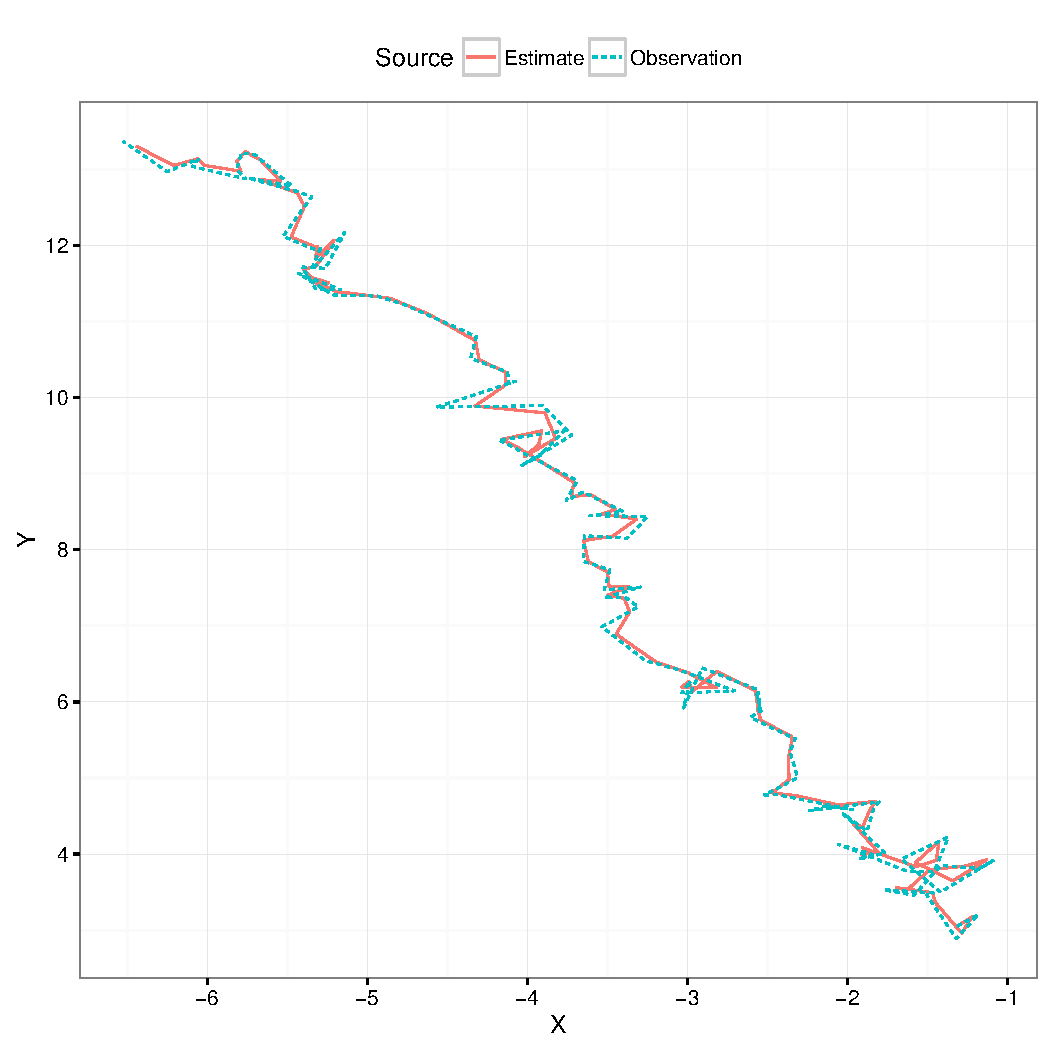
\includegraphics[width=\linewidth]{prg/pf}
  \caption{A simple particle filter}
  \label{fig:pf}
\end{figure}

Before diving into the details of the implementation of \verb|PFState|, etc.,
we will first define a few constants and types. The state space is of dimension
$4$. And it is natural to use a \verb|StateMatrix| as the base class of
\verb|PFState|,
\begin{Verbatim}
  using PFStateBase = StateMatrix<RowMajor, 4, double>;
\end{Verbatim}
We define the following constants as the indices of each state component.
\begin{Verbatim}
  static constexpr std::size_t PosX = 0;
  static constexpr std::size_t PosY = 1;
  static constexpr std::size_t VelX = 2;
  static constexpr std::size_t VelY = 3;
\end{Verbatim}

\subsubsection{State: \texttt{PFState}}

As noted earlier, \verb|StateMatrix| will be used as the base class of
\verb|PFState|. Since the data will be shared by all particles, we also store
the data within this class. And methods will be provided to read the data from
an external file, and compute the log-likelihood $\ell(X^{(i)})$, which
accesses the data. Below the declaration of the class \verb|PFState| is shown,
\begin{Verbatim}
  class PFState : public PFStateBase
  {
      public:
      using PFStateBase::PFStateBase;

      // Return $\ell(X_t^{(i)}|Y_t)$
      double log_likelihood(std::size_t t, size_type i) const;

      // Read data from an external file
      void read_data(const char *param);

      private:
      Vector<double> obs_x_;
      Vector<double> obs_y_;
  };
\end{Verbatim}

\subsubsection{Initialization: \texttt{PFInit}}

The initialization step is implemented as below,
\begin{Verbatim}
  class PFInit
  {
      public:
      std::size_t operator()(Particle<PFState> &particle, void *param)
      {
          eval_param(particle, param);
          eval_pre(particle);
          std::size_t acc = 0;
          for (auto sp : particle)
              acc += eval_sp(sp);
          eval_post(particle);

          return acc;
      }

      void eval_param(Particle<PFState> &particle, void *param)
      {
          particle.value().read_data(static_cast<const char *>(param));
      }

      void eval_pre(Particle<PFState> &particle)
      {
          weight_.resize(particle.size());
      }

      std::size_t eval_sp(SingleParticle<PFState> sp)
      {
          NormalDistribution<double> norm_pos(0, 2);
          NormalDistribution<double> norm_vel(0, 1);
          sp.state(PosX) = norm_pos(sp.rng());
          sp.state(PosY) = norm_pos(sp.rng());
          sp.state(VelX) = norm_vel(sp.rng());
          sp.state(VelY) = norm_vel(sp.rng());
          weight_[sp.id()] = sp.particle().value().log_likelihood(0, sp.id());

          return 0;
      }

      void eval_post(Particle<PFState> &particle)
      {
          particle.weight().set_log(weight_.data());
      }

      private:
      Vector<double> weight_;
  };
\end{Verbatim}
An object of this class is convertible to \verb|Sampler<PFState>::init_type|.
In the main method, \verb|operator()|, \verb|eval_param| is called first to
initialize the data. Then \verb|eval_pre| is called to allocated any resource
this class need before calling any \verb|eval_sp|. In this case, it allocate
the vector \verb|weight_| for storing weights computed later. Next, the main
loop initializes each state component with the respective Gaussian
distribution, computes the log-likelihood and store them in the vector
allocated in the last step. This is done by calling the \verb|eval_sp| method.
After all particles have been initialized, we set the weights of the system in
\verb|eval_post|. Later in section~\ref{sec:Symmetric multiprocessing}, it will
become clear why we structured the implementation this way.

\subsubsection{Move: \texttt{PFMove}}

The move step is similar to the initialization. We show the declaration here,
\begin{Verbatim}
  class PFMove
  {
      public:
      std::size_t operator()(std::size_t t, Particle<PFState> &particle);
      void eval_pre(std::size_t t, Particle<PFState> &particle);
      std::size_t eval_sp(std::size_t t, SingleParticle<PFState> sp);
      void eval_post(std::size_t t, Particle<PFState> &particle);

      private:
      Vector<double> w_;
  };
\end{Verbatim}

\subsubsection{Monitor: \texttt{PFEval}}

Last we define \verb|PFEval|, which simply copies the values of the positions.
\begin{Verbatim}
  class PFEval
  {
      public:
      void operator()(std::size_t t, std::size_t dim,
          Particle<PFState> &particle, double *r)
      {
          eval_pre(t, particle);
          for (std::size_t i = 0; i != particle.size(); ++i, r += dim)
              eval_sp(t, dim, particle.sp(i), r);
          eval_post(t, particle);
      }

      void eval_pre(std::size_t t, Particle<PFState> &particle) {}

      void eval_sp(std::size_t t, std::size_t dim,
          SingleParticle<PFState> sp, double *r)
      {
          r[0] = sp.state(PosX);
          r[1] = sp.state(PosY);
      }

      void eval_post(std::size_t t, Particle<PFState> &particle) {}
  };
\end{Verbatim}

\section{Symmetric multiprocessing}
\label{sec:Symmetric multiprocessing}

The above example is implemented in a sequential fashion. However, the loops
inside \verb|PFInit|, \verb|PFMove| and \verb|PFEval| clearly can be
parallelized. The library provides basic support of multicore parallelization
through its \smp module. Two widely used backends, OpenMP and \tbb are
available. Here we demonstrate how to use the \tbb backend. First we will
declare the implementation classes as derived classes,
\begin{Verbatim}
  class PFInit : public InitializationTBB<PFState>;
  class PFMove : public MoveTBB<PFState>;
  class PFEval : public MonitorEvalTBB<PFState>;
\end{Verbatim}
And remove \verb|operator()| from their implementations. After these changes,
the implementation will be parallelized using \tbb. The complete program can be
found in section The complete program is shown in
appendix~\appref{app:sub:Parallelized implementation using TBB}.

It works as if \verb|InitializationTBB<PFState>| has an implementation of
\verb|operator()| as we did before, except it is parallelized. Now it is clear
that, method such as \verb|eval_pre| and \verb|eval_post| are called before and
after the main loop. Method \verb|eval_sp| is called within the loop and it
need to be thread-safe if called with different arguments. This is the main
reason we constructed the \verb|NormalDistribution| objects within
\verb|eval_sp| instead of as member data, even though they are constructed in
exactly the same way for each particle. This is because
\verb|NormalDistribution::operator()| is a mutable method and thus not
thread-safe. If any of these member functions does not do anything, then it
does not have to be defined in the derived class.

Apart from the three base classes we have shown here, there are also
\verb|InitializationOMP|, etc., for using the OpenMP backend. And
\verb|InitializationSEQ|, etc., for implementation without parallelization. The
later works in exactly the same way as our implementation in the last section.
It is often easier to debug a single-threaded program than a parallelized one.
And thus one may develop the algorithm with the sequential backend and obtain
optimal performance latter by only changing the name of a few base class names.
This can usually be done automatically through a build system.

\subsection{Performance consideration}
\label{sec:Performance consideration}

The base classes dispatch calls to \verb|eval_pre|, \verb|eval_sp|, etc.,
through the virtual function mechanism. The performance impact is minimal for
\verb|eval_pre| and \verb|eval_post|, since they are called only once in each
iteration and we expect the computational cost will be dominated by
\verb|eval_sp| in most cases. However, the dynamic dispatch can cause
considerable performance degenerating if the cost of a single call to
\verb|eval_sp| is small while the number of particles is large. Modern
optimizing compilers can usually devirtualize the method calls in trivial
situations. However, it is not always possible. In this situation, the library
will need a little help from the user to make compile-time dispatch. For each
implementation class, we will declare it in the following way,
\begin{Verbatim}
  class PFInit : public InitializationTBB<PFState, PFInit>;
  class PFMove : public MoveTBB<PFState, PFMove>;
  class PFEval : public MonitorEvalTBB<PFState, PFEval>;
\end{Verbatim}
The second template argument of the base class need to be exactly the same as
the derived class. For interested users, this is called Curiously Recurring
Template
Pattern\footnote{\url{https://en.wikipedia.org/wiki/Curiously_recurring_template_pattern}}
(\crtp). This usage of the library's base classes also provides other
flexibility. The methods \verb|eval_pre| etc., can be either \verb|const| or
mutable. They can also be \verb|static|.
